% !TEX root =  ../appendix.tex
\section{Personalized Schedules for Measurement of SCr}
\label{sec: simulation_study}
Currently, the schedule for measurement of SCr levels and fixed and common for all patients. SCr levels are measured 20 times in the first year after transplantation and every three months thereafter. Instead of a common fixed schedule for all patients, we propose using a different schedule for every patient. More specifically, we propose using personalized schedules based on joint models \citet{drizopoulosPersScreening}. Since the SCr measurements are already taken for the kidney transplant patients, in order to demonstrate the efficacy of the personalized schedules we conduct a small simulation. To this end, we first assume a population of kidney transplant patients, whose SCr and hazard of graft failure follow a JM of the form described in \ref{sec : jm_amctx}, with parameters equal to the posterior mean of parameters estimated from the joint model fitted to the kidney transplant dataset. From this population we sample 625 patients, which are further split into a training (575 patients) and test (50 patients) part. For the training patients we generate a graft failure time $T^*_i$ as well as a random and non-informative censoring time $C_i$. For the test patients the graft failure time $T^*_j$ and an intervention time $T^I_j$ is generated. The intervention time is the time at which the 6 month dynamic risk of graft failure of the patient becomes larger than a certain threshold $\kappa$. The choice of $\kappa$ dictates the amount of time at hand between intervention and graft failure. In this simulation we evaluate two $\kappa$ values, namely 0.05 and 0.025. While the results for $\kappa = 0.05$ are presented in the main manuscript, here we present results for $\kappa = 0.025$. We fit a joint model of the specification described in Section \ref{sec : jm_amctx} to the training data set and obtain a MCMC sample from the posterior distribution of the parameters of the JM. Using the fitted JM, we then iteratively schedule SCr measurements for the test patients, until the dynamic risk of graft failure \citep{rizopoulos2011dynamic} of the patients becomes larger than the threshold $\kappa$. Let $N^I_j$ denote the number of SCr measurements conducted for the $j$-th test patient. The time difference between the observed intervention time due to the schedule ($T^S_j$) and the true intervention time, that is, the intervention offset is denoted by $O^I_j = T^S_j - T^I_j$. Lastly, the failure offset $O^*_j = T^S_j - T^*j$ is the time at hand between the observed intervention time and the time of graft failure. Using the test patients, we calculate these measures for both personalized and fixed schedules. It is to be noted that in the ideal scenario, $N^I_j$ will be one, and offset $O^I_j$ will be zero. 

A boxplot of the observed values of the number of SCr measurements $N^I_j$, intervention offset $O^I_j$ and failure offset $O^*_j$ are presented in Figure \ref{fig : nObspt025}, Figure \ref{fig : truethrestimept025} and Figure \ref{fig : truestoptimept025}, respectively. An advantage of using 2.5\% risk over 5\% risk is that the risk of overshooting the true graft failure time is less due to less risk being taken. In this scenario, although the personalized schedule conducts less SCr measurements, it also exceeds the true intervention time more often than the fixed schedule.

\begin{figure}[!htb]
\centerline{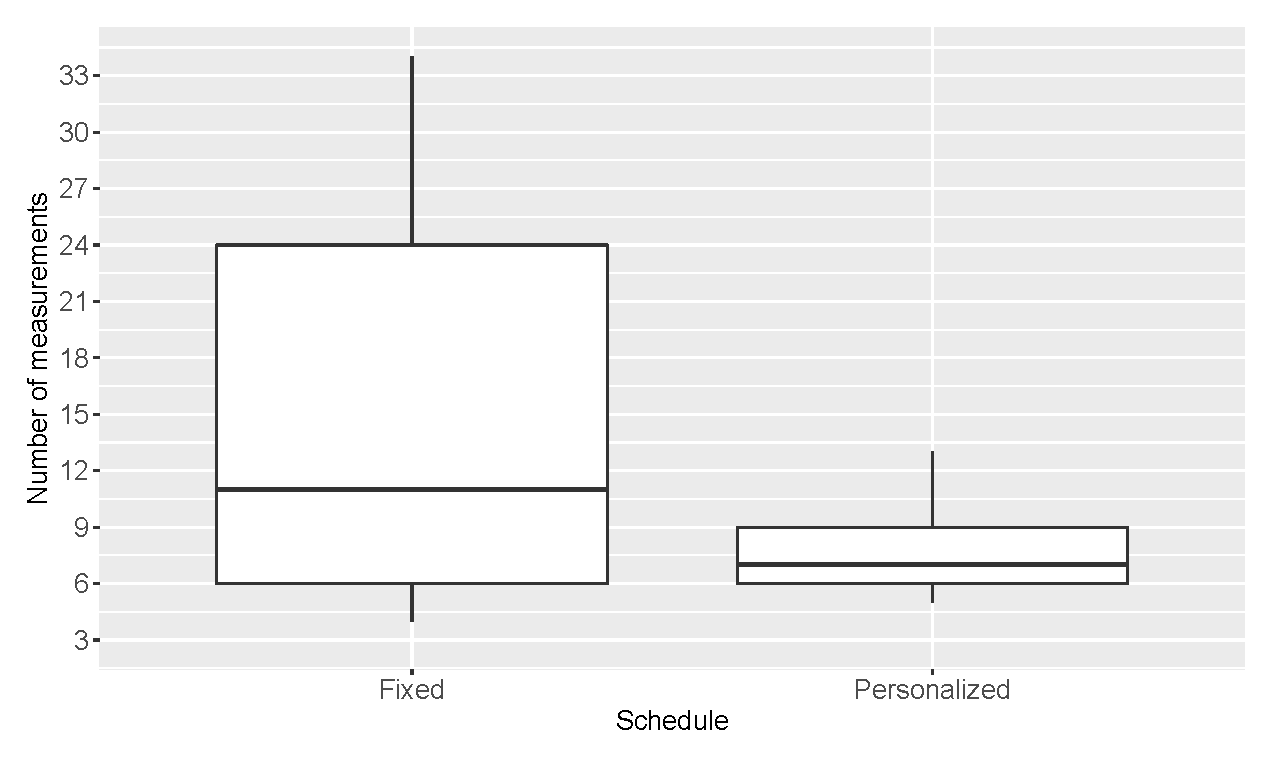
\includegraphics[width=\columnwidth]{images/nObspt025.eps}}
\caption{Boxplot of the number of SCr measurements $N^I_j$ for the test patients, for $\kappa = 0.025$.}
\label{fig : nObspt025}
\end{figure}

\begin{figure}[!htb]
\centerline{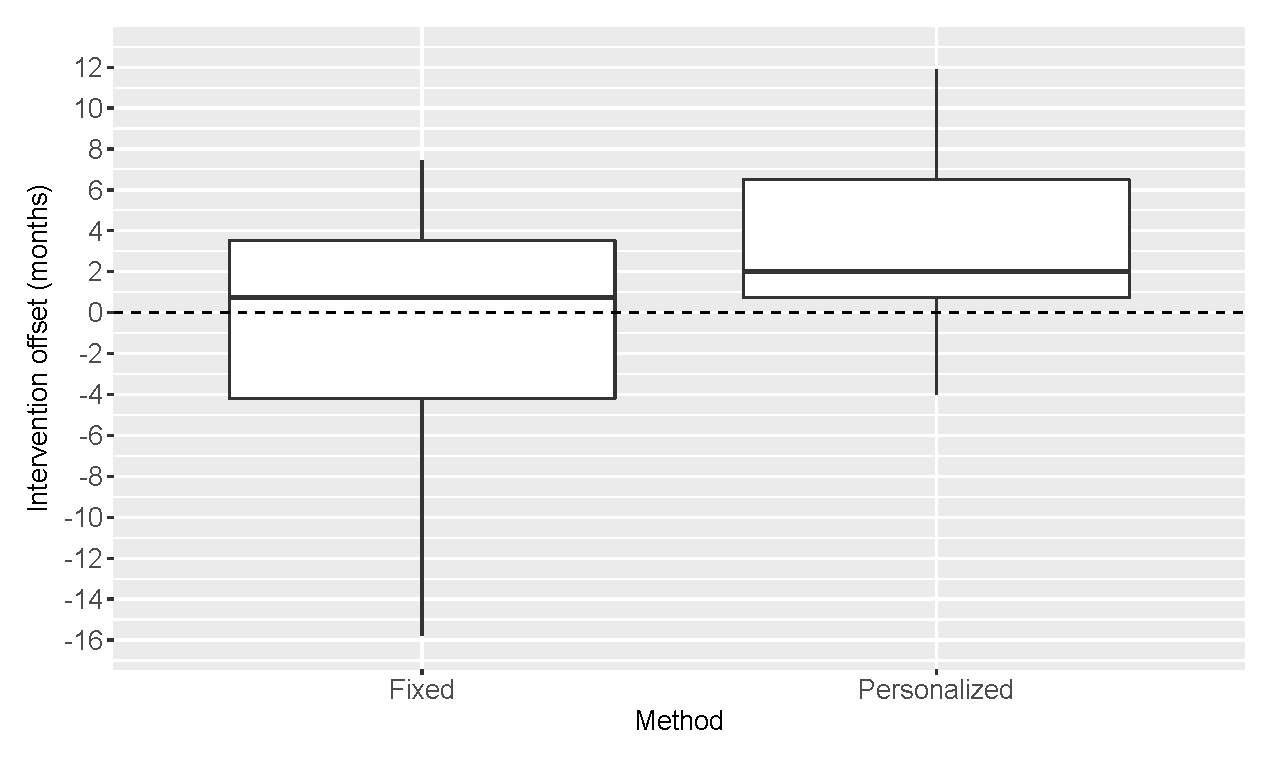
\includegraphics[width=\columnwidth]{images/truethrestimept025.eps}}
\caption{Boxplot of the intervention offset $O^I_j$ for the test patients, for $\kappa = 0.025$. The zero offset mark is displayed with the dashed line.}
\label{fig : truethrestimept025}
\end{figure}

\begin{figure}[!htb]
\centerline{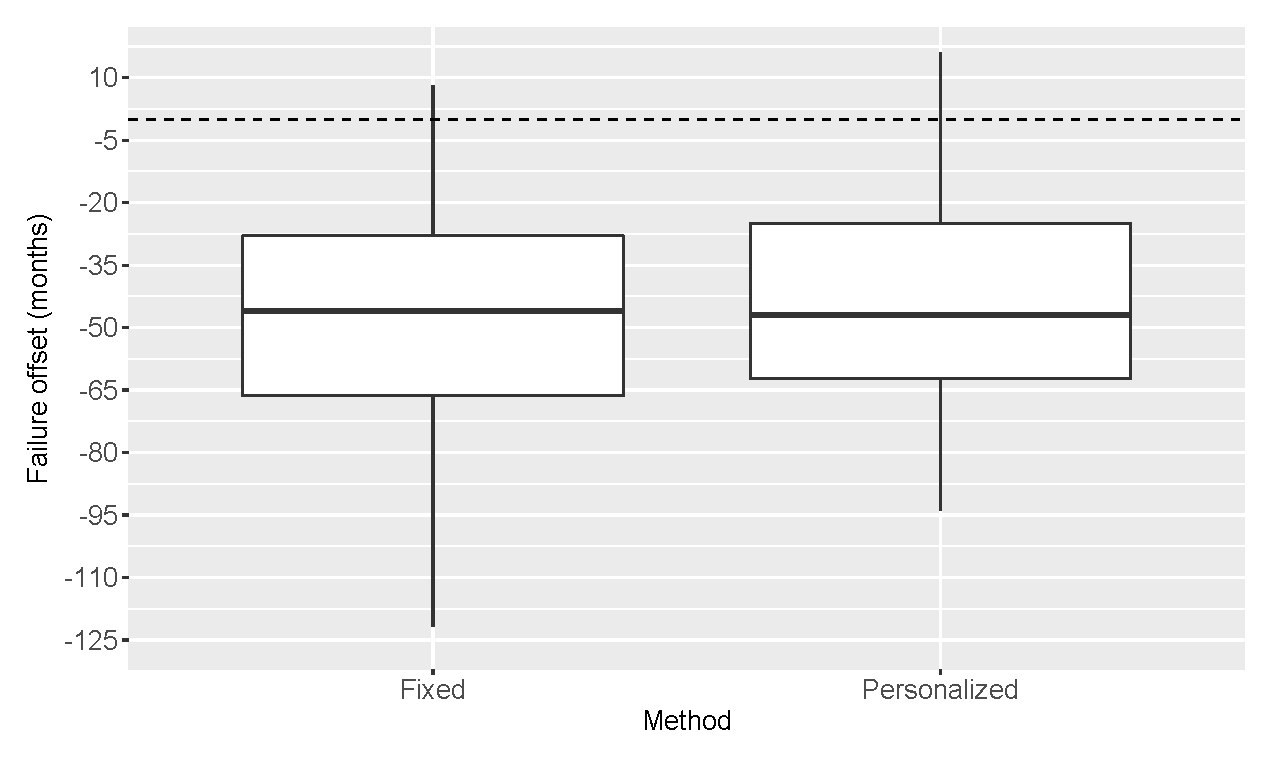
\includegraphics[width=\columnwidth]{images/truestoptimept025.eps}}
\caption{Boxplot of the failure offset $O^*_j$ for the test patients, for $\kappa = 0.025$. The zero offset mark is displayed with the dashed line.}
\label{fig : truestoptimept025}
\end{figure}